\chapter{Web ngữ nghĩa - Semantic Web}
\paragraph{Giới thiệu}
Semantic Web được các nhà nghiên cứu kỳ vọng sẽ trở thành Web 3.0, với đặc trưng riêng biệt là phương thức liên kết dữ liệu (linked data) giữa các hệ thống hoặc các thực thể cho phép thể hiện được nhiều hơn, và rõ ràng hơn mối liên kết giữa các dữ liệu trên mạng lưới web toàn cầu. Cụ thể hơn, Semantic Web có khả năng chuyển đổi văn bản HTML của con người (human readable HTML documents) sang ngôn ngữ máy tính (machine readable documents), giúp cho máy tính làm được nhiều công việc suy nghĩ hơn cho con người \cite{semantic1}.
\\
Ngày nay, đa phần dữ liệu trên web được cung cấp dưới dạng trang web (web pages) - văn bản HTML được liên kết với nhau bằng các liên kết (hyperlinks). Cả người và máy tính đều có thể dễ dàng đọc hiểu những văn bản đó, tuy nhiên thay vì tìm kiếm những từ khoá trong trang web, máy tính lại gặp trở ngại khi chọn lọc những ý nghĩa trong các văn bản đó. Một trang web chứa rất nhiều thông tin, nhưng những thông tin đó không phải là những thông tin thô - mà chỉ là những văn bản HTML được xây dựng từ cơ sở dữ liệu.
\begin{itemize}
\item Chuyển những trang web dữ liệu thành những tiến trình xử lý thông minh nhân tạo (giúp trang web phải “suy nghĩ” để xử lý giúp con người).
\item Khuyến khích các công ty, các doanh nghiệp và các cá nhân trình bày dữ liệu tự do hơn, theo một quy chuẩn mở.
\item Khuyến khích các doanh nghiệp sử dụng dữ liệu đã có sẵn trên web.
\end{itemize}

\section{Semantic Web dựa trên giả định thế giới mở (OWA)} 
Như chúng ta đã biết thì về mục tiêu mà Semantic Web hướng đến, để đạt được những mục tiêu đó, cần có khả năng xử lý thông tin ở khắp mọi nơi đòi hỏi các tiêu chuẩn cũng như các nguyên lý tổ chức dữ liệu sẽ không giống như trước (khi chúng ta vẫn còn tổ chức dữ liệu thành các bảng dữ liệu quan hệ) theo giả định thế giới đóng. Do đó với tính chất muốn bao quát hết tất cả thông tin trên web ( gồm luôn những thông tin chưa đầy đủ - imcomplete information) thì Semantic Web đã lấy Giả định Thế Giới Mở (có thể xem ở phụ lục thêm A) nhằm đảm bảo một hệ thống luôn sẵn sàng mở rộng và tiếp nhận thông tin mới mà không đòi hỏi phải thiết kế lại.
\\
Một so sánh ngắn gọn giữa giả định Thế Giới Mở (Open World Assumption - OWA)\cite{OWA_0} được Semantic Web chấp nhận và giả định Thế Giới Đóng (Closed World Assumption - CWA).
\begin{description}
	\item[Closed World Assumption] 
	Giả định Thế Giới Đóng (CWA) là giả định mà những điều không chắc hoặc không có cơ sở để chứng minh là \textbf{đúng} sẽ được chấp nhận là \textbf{sai}.
	\item[Open World Assumption]
	Giả định Thế Giới Mở (OWA) thì ngược lại, với những điều không chắc hoặc không có cơ sở để chứng minh là \textbf{đúng} sẽ được chấp nhận là \textbf{chưa biết}. 
	\item[Ví dụ]
	Xem xét một câu nói sau đây: "A là một công dân của nước Hoa Kỳ". Nếu có ai đó hỏi "A có phải là một công dân của Việt Nam hay không ?". Xét theo CWA, câu trả lời là \textit{không}, ngược lại với OWA thì câu trả lời là \textit{chưa biết}. 
\end{description}
\section{Các tiêu chuẩn và thành phần của Semantic Web}
Khái niệm "Semantic Web" thường được sử dụng cụ thể hơn nhằm chỉ đến những định dạng và công nghệ để hiện thực hóa nó. Việc tổ chức, tập hợp và phục hồi dữ liệu liên kết thực hiện được nhờ vào các công đặc tả chính thức về các khái niệm, định nghĩa và mối quan hệ trong một vùng tri thức (knowledge domain) cho trước. Tất cả các công nghệ này đều được quy định thành một tiêu chuẩn của W3C \cite{semantic2}. Các tiêu chuẩn được liệt kê dưới đây
\begin{figure}[h!]
	\centering
	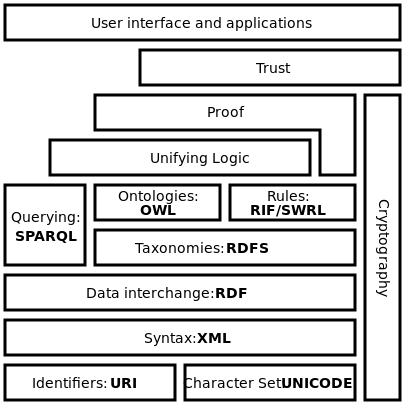
\includegraphics[width=110mm]{Figures/semantic_web_stack.png}
	\caption{The Semantic Web Stack \label{overflow}}
\end{figure}
\begin{itemize}
\item \href{http://en.wikipedia.org/wiki/Resource\_Description\_Framework}{Resource Description Framework}, một phương thức chung để biểu diễn thông tin cho semantic web.
\item \href{http://en.wikipedia.org/wiki/RDF_Schema}{RDF Schema}
\item \href{http://en.wikipedia.org/wiki/Simple_Knowledge_Organization_System}{Simple Knowledge Organization System} (SKOS)
\item \href{http://en.wikipedia.org/wiki/SPARQL}{SPARQL} - Ngôn ngữ truy vấn dữ liệu biểu diễn dưới dạng RDF.
\item \href{http://en.wikipedia.org/wiki/Notation3}{Notation3}, thiết kế với tiêu chí hiểu được bởi con người.
\item \href{http://en.wikipedia.org/wiki/N-Triples}{N-Triples}, một định dạng dùng để lưu và truyền dữ liệu.
\item \href{http://en.wikipedia.org/wiki/Turtle_(syntax)}{Turtle} (Terse RDF Triple Language)
\item \href{http://en.wikipedia.org/wiki/Web_Ontology_Language}{Web Ontology Language} (OWL), một họ các ngôn ngữ biểu diễn tri thức
\item \href{}{Rule Interchange Format} (RIF), một framework chung của các ngôn ngữ điều luật web hỗ trợ chuyển đổi nhiều điều luật khác nhau trên web
\end{itemize}

Hình Semantic Web Stack\cite{semantic3} miêu tả kiến trúc của Semantic Web:

\begin{itemize}
\item XML cung cấp một cú pháp cơ bản nhất cho nội dung bên trong tài liệu, và không có liên quan ngữ nghĩa gì đến nội dung ngữ nghĩa mà nội dụng nó chứa. XML không phải là một thành phần cần thiết trong các công nghệ Semantic Web trong hầu hết các trường hợp, tồn tại cú pháp thay thế khác như Turle \textsuperscript{*}. 
\item XML Schema là một ngôn ngữ dùng để cung cấp và hạn chế cấu trúc nội dung của các thành phần nằm trong tài liệu XML, nói cách khác nó giúp chúng ta dạnh nói dung mà tài liệu đó chưa là gì. Ví dụ: OWL/XML vs. RDF/XML
\item RDF \cite{rdf} là một ngôn ngữ đơn giản dùng để diễn tả các mô hình dữ liệu (ở đây muốn chỉ đến các nguồn dữ liệu web) và mối quan hệ của chúng. Một mô hình dự theo RDF có thể được biểu diễn bằng nhiều cú pháp khác nhau, vd: RDF/XML, N3, Turtle và RDFa. Có thể nói RDF chính là thành phần cơ bản và quan trọng nhất của Semantic Web.
\item RDF Schema \cite{rdfs} mở rộng RDF và là từ vựng để đặc tả các thuộc tính và lớp trong các tài nguyên dựa trên RDF, với ngữ nghĩa dựa trên các việc tạo ra nhiều phân cấp lớp và thuộc tính.
\item OWL thêm nhiều từ vựng hơn để diễn các thuộc  tính và lớp, và điểm quan trọng là nó thêm các từ vựng để đặc tả mối quan hệ giữa các lớp với nhau, vd: ranh giới riêng biệt giữa các lớp với nhau (disjointness), các quy định với số lượng (cardinality), cung cấp nhiều loại dữ liệu cho các thuộc tính, và các đặc tính của các thuộc tính (vd: đối xứng/ bất đối xứng, và các lớp liệt kê.
\item SPARQL là một giao thức và ngôn ngữ truy vấn dữ liệu dành cho tài nguyên của semantic web.
\item RIF (W3C Rule Interchange Format) là một ngữ ngữ XML để biểu diễn điều luật web mà máy tính có thể thực thi.
\end{itemize}
{\let\thefootnote\relax\footnotetext{*\textit{
			Turtle: http://en.wikipedia.org/wiki/Turtle\_(syntax)}}
}
\paragraph{Kết luận} Trên đây chúng em chỉ liệt kê những thành phần và tiêu chuẩn cơ bản nhất mà tổ chức W3C đã vạch ra nhằm xây dựng một mô hình Web ngữ nghĩa của tương lai. Nội dung để tài của chúng em chỉ hạn chế trong việc nghiên cứu và khai thác ngôn ngữ ontology web nhằm khai thác tiềm năng về mặc ngữ nghĩa (suy luận ra những thông tin mới dựa trên những suy luận từ ngữ nghĩa của những thông tin được khai báo) nhằm phục vụ cho việc phân loại thông qua các thuộc tính của sản phẩm. Chương kế tiếp sẽ đi qua tìm hiểu về Ontology Web Language(OWL) và Semantic Web Rule Language (SWRL) hai thành phần chính giúp hình thành khả năng phần loại tự động của đề tài này.




